\section{Appendix}


\subsection{Devices Seen}


\subsection{Link Utilization}

\begin{figure}[t]
  \begin{minipage}{\linewidth}
  \includegraphics[width=0.98\linewidth]{figures/bytesperdevice/device_utilization_entire_data}
  \caption{Device utilization for the entire two weeks period. We see that more than a third of the total traffic is by Apple(iOS) devices. This may be due to the fact that Windows/Android devices are made by multiple manufacturers.}
  \label{fig:countofdevices}
  \end{minipage}
\end{figure}

\begin{figure}[t]
  \begin{minipage}{\linewidth}
  \subfloat[Diurnal Uplink Home 5]{
  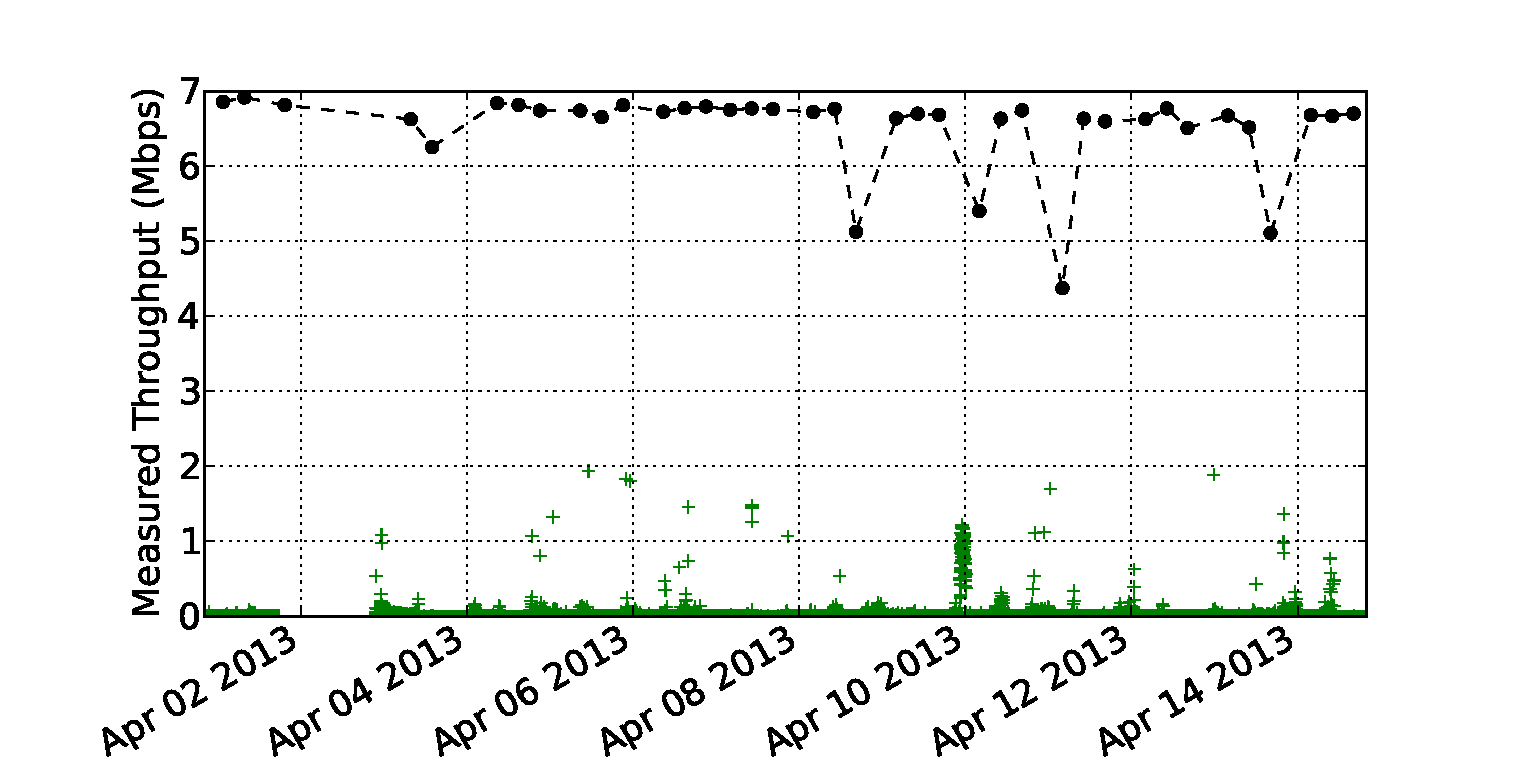
\includegraphics[width=0.98\linewidth]{figures/bitrate/diurnal-usage/5_OW4C60DED0F74B_up}
  \label{fig:diurnal-util-uplink-5}}\\
  \subfloat[Diurnal Downlink Home 5]{
  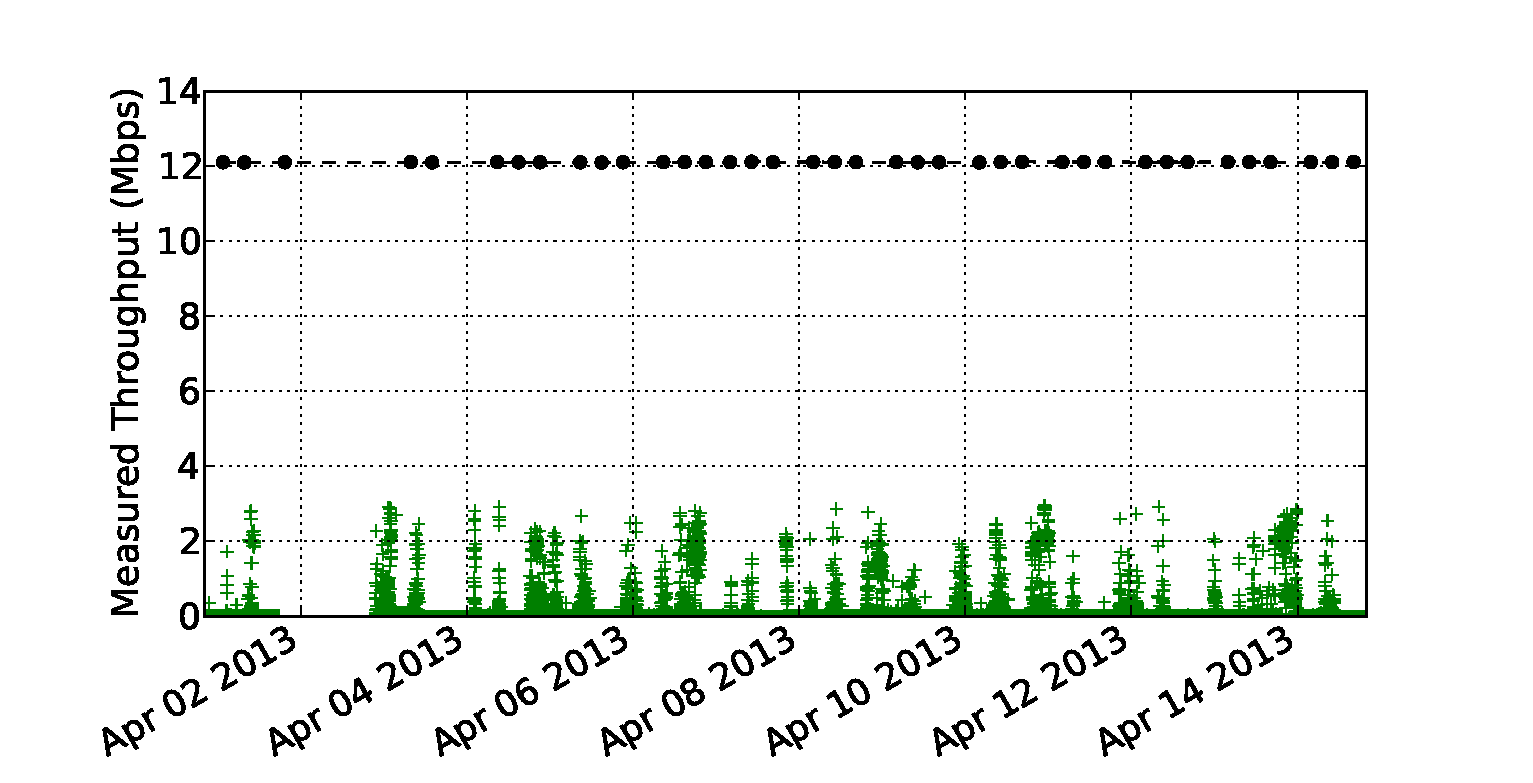
\includegraphics[width=0.98\linewidth]{figures/bitrate/diurnal-usage/5_OW4C60DED0F74B_dw}
  \label{fig:diurnal-util-downlink-5}}\\
  \caption{Diurnal pattern of link utilization for home 5}
  \label{fig:diurnal-util-5}
  \end{minipage}
\end{figure}

\begin{figure}[t]
  \begin{minipage}{\linewidth}
  \subfloat[Diurnal Uplink Home 8]{
  \includegraphics[width=0.98\linewidth]{figures/bitrate/diurnal-usage/8_OWC43DC7B0CAB6_up}
  \label{fig:diurnal-util-uplink-8}}\\
  \subfloat[Diurnal Downlink Home 8]{
  \includegraphics[width=0.98\linewidth]{figures/bitrate/diurnal-usage/8_OWC43DC7B0CAB6_dw}
  \label{fig:diurnal-util-downlink-8}}\\
  \caption{Diurnal pattern of link utilization for home 8}
  \label{fig:diurnal-util-8}
  \end{minipage}
\end{figure}

\begin{figure}[t]
  \begin{minipage}{\linewidth}
  \subfloat[Diurnal Uplink Home 11]{
  \includegraphics[width=0.98\linewidth]{figures/bitrate/diurnal-usage/11_OW4C60DEE6B01C_up}
  \label{fig:diurnal-util-uplink-11}}\\
  \subfloat[Diurnal Downlink Home 11]{
  \includegraphics[width=0.98\linewidth]{figures/bitrate/diurnal-usage/11_OW4C60DEE6B01C_dw}
  \label{fig:diurnal-util-downlink-11}}\\
  \caption{Diurnal pattern of link utilization for home 11}
  \label{fig:diurnal-util-11}
  \end{minipage}
\end{figure}  
  
\begin{figure}[t]
  \begin{minipage}{\linewidth}
  \subfloat[Diurnal Uplink Home 16]{
  \includegraphics[width=0.98\linewidth]{figures/bitrate/diurnal-usage/16_OWC43DC79DE0F7_up}
  \label{fig:diurnal-util-uplink-16}}\\
  \subfloat[Diurnal Downlink Home 16]{
  \includegraphics[width=0.98\linewidth]{figures/bitrate/diurnal-usage/16_OWC43DC79DE0F7_dw}
  \label{fig:diurnal-util-downlink-16}}\\ 
  \caption{Diurnal pattern of link utilization for home 16. Black markers denote active capacity
  estimates and green markers denote the passive measurement: max bits transferred per second in
  a minute. Units are bits per second (bps).}
  \label{fig:diurnal-util-16}
  \end{minipage}
\end{figure}

Figure ~\ref{fig:diurnal-util-5}, ~\ref{fig:diurnal-util-8}, ~\ref{fig:diurnal-util-11},
~\ref{fig:diurnal-util-16} shows that we observe a diurnal usage pattern for link activity.
Peak transfers occur in the evening and night, and some data is transferred in mornings. At
other times the link remains idle. This pattern of usage seen in half of the American homes
running \passive{} is very similar to the connectivity pattern of access points observed for
gateways in \developing{} countries such as India and China (Figure ~\ref{fig:china-availability})


\subsection{Top Domains}


\subsection{Device Utilization}

\begin{figure}[t]
  \includegraphics[width=1.05\linewidth]{figures/device_utilization}
  \caption{Device use fraction. Different markers for different homes. Color denotes type of device.}
  \label{fig:dev-util}
\end{figure}

Figure~\ref{fig:dev-util} plots the ratio of data used by a particular device in a home.

\subsection{Heartbeat}

\begin{figure}[t]
  \includegraphics[width=0.98\linewidth]{figures/outages_scatter_april}
  \caption{Red markers are developed nations, blue are developing}
  \label{fig:outage-scatter}
\end{figure}
